% --------------------------------------
% Document Class
% --------------------------------------
\documentclass[a4paper,11pt]{article}
% --------------------------------------



% --------------------------------------
% Use Package
% --------------------------------------


%\usepackage[francais]{babel}
%\usepackage{ucs}
\usepackage[utf8]{inputenc}
\usepackage[T1]{fontenc}

\usepackage{makeidx}
\usepackage{color}
\usepackage{graphicx}
\usepackage{float}
\usepackage[hidelinks]{hyperref} 
\usepackage{geometry}
%\usepackage{lastpage}
%\usepackage{marginnote}
\usepackage{fancyhdr}
%\usepackage{titlesec}
%\usepackage{framed}
\usepackage{amsmath}
\usepackage{empheq}
\usepackage{array}
\usepackage{multicol}
\usepackage{csquotes}
%\usepackage{adjustbox}

% insert code
\usepackage{listings}

% define our color
\usepackage{xcolor}

% code color
\definecolor{ligthyellow}{RGB}{250,247,220}
\definecolor{darkblue}{RGB}{5,10,85}
\definecolor{ligthblue}{RGB}{1,147,128}
\definecolor{darkgreen}{RGB}{8,120,51}
\definecolor{darkred}{RGB}{160,0,0}

% other color
\definecolor{ivi}{RGB}{141,107,185}

\def\verticaltext#1{\rotatebox[origin=c]{90}{\x{#1}}}


\lstset{
    language=C++,
    captionpos=b,
    extendedchars=true,
    frame=lines,
    numbers=left,
    numberstyle=\tiny,
    numbersep=5pt,
    keepspaces=true,
    breaklines=true,
    showspaces=false,
    showstringspaces=false,
    breakatwhitespace=false,
    stepnumber=1,
    showtabs=false,
    tabsize=3,
    basicstyle=\small\ttfamily,
    backgroundcolor=\color{ligthyellow},
    keywordstyle=\color{ligthblue},
    morekeywords={include, printf, uchar},
    identifierstyle=\color{darkblue},
    commentstyle=\color{darkgreen},
    stringstyle=\color{darkred},
}


% --------------------------------------



% --------------------------------------
% Page setting
% --------------------------------------
%\pagestyle{empty}
\setlength{\headheight}{15pt}

\setcounter{secnumdepth}{3}
\setcounter{tocdepth}{2}

\makeatletter
\@addtoreset{chapter}{part}
\makeatother 

\hypersetup{         % parametrage des hyperliens
  colorlinks=true,      % colorise les liens
  breaklinks=true,      % permet les retours à la ligne pour les liens trop longs
  urlcolor= blue,       % couleur des hyperliens
  linkcolor= black,     % couleur des liens internes aux documents (index, figures, tableaux, equations,...)
  citecolor= green      % couleur des liens vers les references bibliographiques
}

% --------------------------------------

% --------------------------------------
% Information
% --------------------------------------
\title{
  \noindent\hrulefill \\
  \vspace{10mm} Compte-rendu TP3 VisA: Rectification épipolaire et stéréovision dense
}

\author{Gaëtan DEFLANDRE}
% --------------------------------------

\definecolor{myColor}{rgb}{0.5, 0.1, 0.75}

% --------------------------------------
% Begin content
% --------------------------------------
\begin{document}


\maketitle

\noindent\hrulefill \\


\section{Introduction}


\newpage

\section{Fonctionnement général}

\begin{figure}[H]
  \centering
  \shortstack{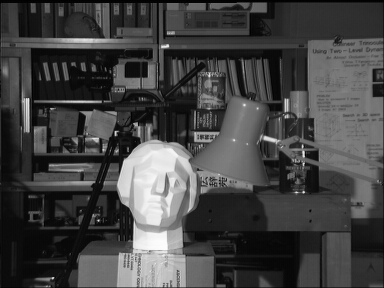
\includegraphics[width=200px]{../left.png} \\ Image de gauche}
  \shortstack{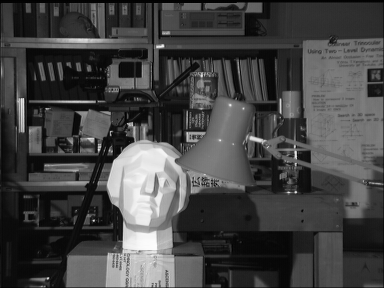
\includegraphics[width=200px]{../right.png} \\ Image de droite}
\end{figure}

La premier double boucle de la fonction initialise la matrice
\textbf{mMinSSD} avec la valeur de $dMinSSD = (2 * iWindowHalfSize + 1)^2 * 512.0$

\begin{lstlisting}[caption=Initialisation]
    // Initialisation de l'image du minimum de SSD
    dMinSSD = pow((double)(2 * iWindowHalfSize + 1), 2.0) * 512.0;
    for (iRow = iWindowHalfSize;
            iRow < mMinSSD.size().height - iWindowHalfSize;
            iRow++)
    {
        // Pointeur sur le debut de la ligne
        pdPtr1 = mMinSSD.ptr<double>(iRow);
        // Sauter la demi fenetre non utilisee
        pdPtr1 += iWindowHalfSize;
        // Remplir le reste de la ligne
        for (iCol = iWindowHalfSize;
                iCol < mMinSSD.size().width - iWindowHalfSize;
                iCol++)
            *pdPtr1++ = dMinSSD;
    }
\end{lstlisting}

Les boucle qui suivent recherche pour chaque pixel de l'image de
gauche le décalage qui minimise la dissimilarité SSD. Les valeurs
des décalages sont stocké dans \textbf{mLeftDisparityMap}.

\section{Calculs des disparités gauches, puis droites}

La fonction \textbf{normalize} est utilisée pour que les images calculées 
utilisent tout l'histogramme des niveaux de gris. Après cela, nous distinguons 
les différents niveaux de gris car l'écart-type est plus élevé.

$$
normalize(mLeftDisparity, mLeftDisparity, 0, 255, CV\_MINMAX);
$$


\begin{figure}[H]
  \centering
  \shortstack{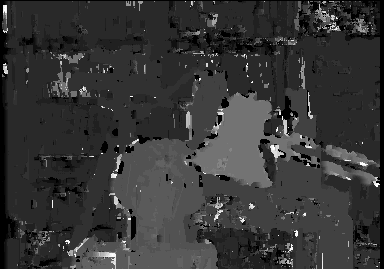
\includegraphics[height=140px]{../left_disparity.png} \\ Disparité de gauche}
  \shortstack{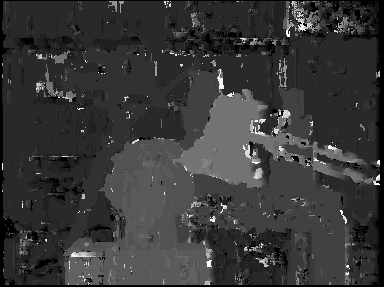
\includegraphics[height=140px]{../right_disparity.png} \\ Disparité de droite}
\end{figure}

\begin{lstlisting}[caption=Calcul du SSD gauche]
    for (unsigned x=iWindowHalfSize; x<=cols; x++){
        for (unsigned y=iWindowHalfSize; y<=rows; y++){
            for (int i= -iWindowHalfSize; i<=iWindowHalfSize; i++){

                if (winX<0 || winX>=cols){
                    // Si on est hors de l'image on passe
                    continue;
                }

                for(int j=-iWindowHalfSize; j<=iWindowHalfSize; j++){

                    winX = x + i;
                    winY = y + j;

                    if (winY<0 || winY>=rows){
                        // Si on est hors de l'image on passe
                        continue;
                    }

                    // Valeur image gauche
                    double il = (double)mLeftGray.at<unsigned char>(winY,winX);
                    // Valeur image droite
                    double ir = (double)mRightGray.at<unsigned char>(winY,winX-iShift);

                    ssd += pow(il-ir, 2.0);

                }
            }

            mLeftSSDCost.at<double>(y,x) = ssd;
            ssd = 0.0;

        }
    }

    return mLeftSSDCost.clone();
\end{lstlisting}

\begin{lstlisting}[caption=Calcul du SSD droit]
    for (unsigned x=iWindowHalfSize; x<=cols; x++){
        for (unsigned y=iWindowHalfSize; y<=rows; y++){
            for (int i= -iWindowHalfSize; i<=iWindowHalfSize; i++){

                if (winX<0 || winX>=cols){
                    // Si on est hors de l'image on passe
                    continue;
                }

                for(int j=-iWindowHalfSize; j<=iWindowHalfSize; j++){

                    winX = x + i;
                    winY = y + j;

                    if (winY<0 || winY>=rows){
                        // Si on est hors de l'image on passe
                        continue;
                    }

                    // Valeur image gauche
                    double il = (double)mLeftGray.at<unsigned char>(winY,winX+iShift);
                    // Valeur image droite
                    double ir = (double)mRightGray.at<unsigned char>(winY,winX);

                    ssd += pow(ir-il, 2.0);

                }
            }

            mRightSSDCost.at<double>(y,x) = ssd;
            ssd = 0.0;

        }
    }

    return mRightSSDCost.clone();
\end{lstlisting}

\section{Cohérence gauche-droite}

\begin{equation}
\begin{aligned}
d_r(x,y) &= d_l(x+d_r(x,y),y) \\
d_l(x,y) &= d_r(x-d_l(x,y),y) \\
\end{aligned}
\end{equation}


\begin{figure}[H]
  \centering
  \shortstack{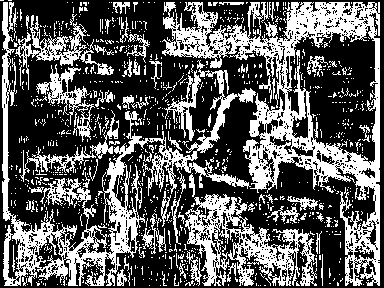
\includegraphics[width=200px]{../mask.png} \\ {\small Masque des disparités cohérente gauche-droite}}
  \shortstack{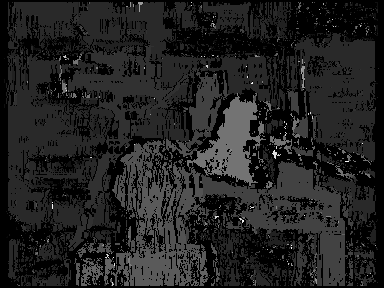
\includegraphics[width=200px]{../disparity.png} \\ {\small Disparité gauche-droite}}
\end{figure}

\begin{lstlisting}[caption=Fonction donnant la disparité cohérente gauche-droite]
/// \brief Verifie la coherence des cartes gauche et froite.
///
/// @param psLeftDisparity: carte gauche des disparites
/// @param psRightDisparity: carte droite des disparites
/// @param psDisparity: carte des disparites fusionnee
/// @param psValidityMask: carte des disparites valides
Mat iviLeftRightConsistency(const Mat& mLeftDisparity,
                            const Mat& mRightDisparity,
                            Mat& mValidityMask)
{
    Mat mDisparity(mLeftDisparity.size(), CV_8U);

    unsigned rows = mLeftDisparity.rows;
    unsigned cols = mLeftDisparity.cols;

    for (unsigned x=0; x<cols; x++) {
        for (unsigned y=0; y<rows; y++) {

            unsigned char dr1 = mRightDisparity.at<unsigned char>(y,x);
            unsigned char dl1 = mLeftDisparity.at<unsigned char>(y,x+dr1);

            unsigned char dl2 = mLeftDisparity.at<unsigned char>(y,x);
            unsigned char dr2 = mRightDisparity.at<unsigned char>(y,x-dl2);

            if(dr1==dl1 && dl2==dr2){
                mValidityMask.at<unsigned char>(y,x) = 0;
                mDisparity.at<unsigned char>(y,x) = dl2;
            } else {
                mValidityMask.at<unsigned char>(y,x) = 255;
                mDisparity.at<unsigned char>(y,x) = 0;
            }
        }
    }

    return mDisparity.clone();
}
\end{lstlisting}

\section{Conclusion}




\end{document}
